\documentclass{article}\usepackage[]{graphicx}\usepackage[]{xcolor}
% maxwidth is the original width if it is less than linewidth
% otherwise use linewidth (to make sure the graphics do not exceed the margin)
\makeatletter
\def\maxwidth{ %
  \ifdim\Gin@nat@width>\linewidth
    \linewidth
  \else
    \Gin@nat@width
  \fi
}
\makeatother

\definecolor{fgcolor}{rgb}{0.345, 0.345, 0.345}
\newcommand{\hlnum}[1]{\textcolor[rgb]{0.686,0.059,0.569}{#1}}%
\newcommand{\hlstr}[1]{\textcolor[rgb]{0.192,0.494,0.8}{#1}}%
\newcommand{\hlcom}[1]{\textcolor[rgb]{0.678,0.584,0.686}{\textit{#1}}}%
\newcommand{\hlopt}[1]{\textcolor[rgb]{0,0,0}{#1}}%
\newcommand{\hlstd}[1]{\textcolor[rgb]{0.345,0.345,0.345}{#1}}%
\newcommand{\hlkwa}[1]{\textcolor[rgb]{0.161,0.373,0.58}{\textbf{#1}}}%
\newcommand{\hlkwb}[1]{\textcolor[rgb]{0.69,0.353,0.396}{#1}}%
\newcommand{\hlkwc}[1]{\textcolor[rgb]{0.333,0.667,0.333}{#1}}%
\newcommand{\hlkwd}[1]{\textcolor[rgb]{0.737,0.353,0.396}{\textbf{#1}}}%
\let\hlipl\hlkwb

\usepackage{framed}
\makeatletter
\newenvironment{kframe}{%
 \def\at@end@of@kframe{}%
 \ifinner\ifhmode%
  \def\at@end@of@kframe{\end{minipage}}%
  \begin{minipage}{\columnwidth}%
 \fi\fi%
 \def\FrameCommand##1{\hskip\@totalleftmargin \hskip-\fboxsep
 \colorbox{shadecolor}{##1}\hskip-\fboxsep
     % There is no \\@totalrightmargin, so:
     \hskip-\linewidth \hskip-\@totalleftmargin \hskip\columnwidth}%
 \MakeFramed {\advance\hsize-\width
   \@totalleftmargin\z@ \linewidth\hsize
   \@setminipage}}%
 {\par\unskip\endMakeFramed%
 \at@end@of@kframe}
\makeatother

\definecolor{shadecolor}{rgb}{.97, .97, .97}
\definecolor{messagecolor}{rgb}{0, 0, 0}
\definecolor{warningcolor}{rgb}{1, 0, 1}
\definecolor{errorcolor}{rgb}{1, 0, 0}
\newenvironment{knitrout}{}{} % an empty environment to be redefined in TeX

\usepackage{alltt}
\usepackage[sc]{mathpazo}
\renewcommand{\sfdefault}{lmss}
\renewcommand{\ttdefault}{lmtt}
\usepackage[T1]{fontenc}
\usepackage{geometry}
\geometry{verbose,tmargin=2.5cm,bmargin=2.5cm,lmargin=2.5cm,rmargin=2.5cm}
\setcounter{secnumdepth}{2}
\setcounter{tocdepth}{2}
\usepackage[unicode=true,pdfusetitle,
 bookmarks=true,bookmarksnumbered=true,bookmarksopen=true,bookmarksopenlevel=2,
 breaklinks=false,pdfborder={0 0 1},backref=false,colorlinks=false]
 {hyperref}
\hypersetup{
 pdfstartview={XYZ null null 1}}

\makeatletter
%%%%%%%%%%%%%%%%%%%%%%%%%%%%%% User specified LaTeX commands.
\renewcommand{\textfraction}{0.05}
\renewcommand{\topfraction}{0.8}
\renewcommand{\bottomfraction}{0.8}
\renewcommand{\floatpagefraction}{0.75}

\makeatother
\IfFileExists{upquote.sty}{\usepackage{upquote}}{}
\begin{document}








The results below are generated from an R script.

\begin{knitrout}
\definecolor{shadecolor}{rgb}{0.969, 0.969, 0.969}\color{fgcolor}\begin{kframe}
\begin{alltt}
\hlkwd{library}\hlstd{(bio3d)}


\hlstd{plot_protein} \hlkwb{<-} \hlkwa{function}\hlstd{(}\hlkwc{protein}\hlstd{)\{} \hlcom{#input is the name of the protein}

  \hlstd{s1} \hlkwb{<-} \hlkwd{read.pdb}\hlstd{(protein)} \hlcom{#reads the protein sequence }
  \hlstd{s1.chainA} \hlkwb{<-} \hlkwd{trim.pdb}\hlstd{(s1,} \hlkwc{chain}\hlstd{=}\hlstr{"A"}\hlstd{,} \hlkwc{elety}\hlstd{=}\hlstr{"CA"}\hlstd{)} \hlcom{#specifies the protein's chain}

  \hlstd{s1.b} \hlkwb{<-} \hlstd{s1.chainA}\hlopt{$}\hlstd{atom}\hlopt{$}\hlstd{b} \hlcom{#extracts the B factor}

  \hlkwd{plotb3}\hlstd{(s1.b,} \hlkwc{sse}\hlstd{=s1.chainA,} \hlkwc{typ}\hlstd{=}\hlstr{"l"}\hlstd{,} \hlkwc{ylab}\hlstd{=}\hlstr{"Bfactor"}\hlstd{)} \hlcom{#plots the residue vs. B factor}
\hlstd{\}}

\hlkwd{plot_protein}\hlstd{(}\hlstr{"4AKE"}\hlstd{)} \hlcom{#sample call to the function}
\end{alltt}
\begin{verbatim}
##   Note: Accessing on-line PDB file
\end{verbatim}


{\ttfamily\noindent\color{warningcolor}{\#\# Warning in get.pdb(file, path = tempdir(), verbose = FALSE): /var/folders/yq/39\_815d11s9csyl2w7tx\_mgc0000gn/T//RtmpTyYZF9/4AKE.pdb \ exists. Skipping download}}\end{kframe}

{\centering 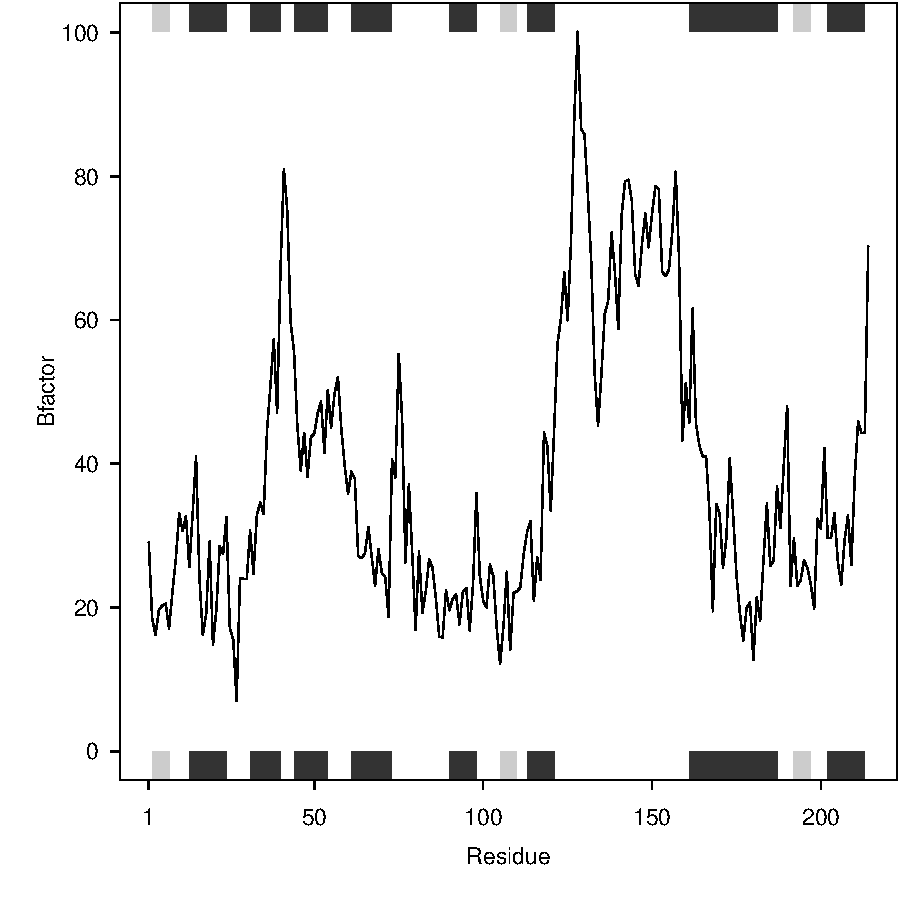
\includegraphics[width=.6\linewidth]{figure/hw06-Rnwauto-report-1} 

}


\end{knitrout}

The R session information (including the OS info, R version and all
packages used):

\begin{knitrout}
\definecolor{shadecolor}{rgb}{0.969, 0.969, 0.969}\color{fgcolor}\begin{kframe}
\begin{alltt}
\hlkwd{sessionInfo}\hlstd{()}
\end{alltt}
\begin{verbatim}
## R version 4.2.1 (2022-06-23)
## Platform: x86_64-apple-darwin17.0 (64-bit)
## Running under: macOS Catalina 10.15.7
## 
## Matrix products: default
## BLAS:   /System/Library/Frameworks/Accelerate.framework/Versions/A/Frameworks/vecLib.framework/Versions/A/libBLAS.dylib
## LAPACK: /Library/Frameworks/R.framework/Versions/4.2/Resources/lib/libRlapack.dylib
## 
## locale:
## [1] en_US.UTF-8/en_US.UTF-8/en_US.UTF-8/C/en_US.UTF-8/en_US.UTF-8
## 
## attached base packages:
## [1] stats     graphics  grDevices utils     datasets  methods   base     
## 
## other attached packages:
## [1] plotly_4.10.0 ggplot2_3.3.6 bio3d_2.4-3  
## 
## loaded via a namespace (and not attached):
##  [1] Rcpp_1.0.9        highr_0.9         pillar_1.8.1      compiler_4.2.1   
##  [5] tools_4.2.1       digest_0.6.29     evaluate_0.16     viridisLite_0.4.1
##  [9] jsonlite_1.8.2    lifecycle_1.0.3   tibble_3.1.8      gtable_0.3.1     
## [13] pkgconfig_2.0.3   rlang_1.0.6       cli_3.4.1         crosstalk_1.2.0  
## [17] yaml_2.3.5        parallel_4.2.1    xfun_0.33         fastmap_1.1.0    
## [21] stringr_1.4.1     knitr_1.40        withr_2.5.0       dplyr_1.0.10     
## [25] httr_1.4.4        generics_0.1.3    vctrs_0.4.2       htmlwidgets_1.5.4
## [29] grid_4.2.1        tidyselect_1.2.0  glue_1.6.2        data.table_1.14.2
## [33] R6_2.5.1          fansi_1.0.3       farver_2.1.1      purrr_0.3.5      
## [37] tidyr_1.2.1       magrittr_2.0.3    scales_1.2.1      htmltools_0.5.3  
## [41] colorspace_2.0-3  labeling_0.4.2    utf8_1.2.2        stringi_1.7.8    
## [45] lazyeval_0.2.2    munsell_0.5.0
\end{verbatim}
\begin{alltt}
\hlkwd{Sys.time}\hlstd{()}
\end{alltt}
\begin{verbatim}
## [1] "2022-10-16 13:53:28 PDT"
\end{verbatim}
\end{kframe}
\end{knitrout}


\end{document}
